\documentclass[10pt,a4paper]{article}
\usepackage{cogsci}

% \documentclass[12pt,a4paper]{article}
% \usepackage[a4paper, total={6.5in, 9in}]{geometry}

\usepackage{pslatex}
\usepackage{apacite}
\usepackage{color}
\usepackage{graphicx}
\usepackage{subcaption}

\newcommand{\todo}[1]{{\color{red}#1}}

\title{Recovering gaps in stories}
 
\author{{\large \bf Erin Bennett} (erindb@stanford.edu) \\ %and
%   {\large {\bf Noah D. Goodman}} (ngoodman@stanford.edu) \\
  Department of Psychology, Stanford University}


\begin{document}

\maketitle


\begin{abstract}

Humans have a great deal of commonsense knowledge -- e.g. about causal relations, abstract roles, and common coocurrances -- that we implicitly use in understanding the world.
This knowledge allows us to fill in gaps in the stories that people tell, inferring other events that likely happened given what a speaker chooses to mention.
Some recent script induction models have been developed to learn commonsense knowledge from natural language corpora.
One common evaluation metric for script induction models is the "narrative cloze task" in which one event from a chain of events described in a corpus is left out for the model to recover.
While this is a reasonable starting point, based in the intuition that humans are able to infer unmentioned events in stories, several sources of information suggest that the task may not be an ideal metric for commonsense knowledge acquisition.
In this paper, we present a pilot experiment which to demonstrate that recovering events that were mentioned in {\em actual} stories may be very difficult for people to do with much accuracy, even with rich linguistic information to draw on.
Our pilot experiments also suggest that agreement among human participants about how to complete a narrative is similarly low, and that even when participants agree with one another, the inferences of an existing script induction model does not appear to track their choices.
In an appendix section, we provide illustrative simulations of very simple domains with handwritten "scripts" and show that events mentioned in an informative story tend to be much less recoverable by a rational listener with domain knowledge than events that are true but not mentioned.

\textbf{Keywords:} 
commonsense knowledge ; script induction ; narrative cloze ; narrative understanding
\end{abstract}

\section{Introduction}

Humans have a great deal of commonsense knowledge that we implicitly use in understanding the world.
This commonsense knowledge includes knowledge about causal relations between events.
For example if a glass falls on the floor, most people would agree that it will probably break.
Commonsense knowledge also involves knowledge about abstract roles that people, places, and things can play in a situation.
For example, if someone is a server at a restaurant, we expect that they ask for orders, bring food, and are paid to be there.
Commonsense knowledge can also refer to the myriad of facts and features that tend to coocur with particular contexts.
For example, when you walk into a restaurant, you expect to see tables, silverware, and possibly a bar.
% %<complete_nonsense>
% Commonsense knowledge might also include factual, relational knowledge, such as the fact that the restaurant Olive Garden serves mostly pasta, or that on Stanford University's campus, Subway is next to Panda Express. However, this more concrete, factual knowledge is currently easier to formally specify and hence more tractable for machines to acquire, than the more abstract knowledge of cause, roles, and features in the previous examples.
% %</complete_nonsense>
Understanding and representing this kind of human knowledge in machines is a long-standing problem in artificial intelligence, and many researchers have thought about this problem and made useful contributions.
% Researchers have been working to operationalize what we mean by commonsense knowledge for many years.
One challenge in operationalizing human commonsense for artificial intelligence is how to evaluate performance of models. In one evaluation method, the narrative cloze task, models must recover a left-out event from a coreference chain in a natural language corpus.
We explore human performance on this task in a pilot experiment, demonstrating that people's performance, and even their agreement with each other, is quite low on these task.
In an appendix section we explore how storytellers' intention to be informative makes the narrative cloze task much more difficult than recovering {\em unmentioned} events, the task that humans are thought to do quite well at and which inspired the narrative cloze task.

\subsection{Background}

\subsubsection{Scripts in Psychology}

Researchers have identified many subtle ways in which human commonsense knowledge comes to play in understanding stories, from which events of a story are more or less memorable to whether a definite (“the”) or indefinite (“a”) article is more appropriate in a given context. One way of articulating commonsense knowledge is that it can be organized into scripts, "structure that describe appropriate sequences of events in a particular context, ... made up of slots and requirements about what can fill those slots," \cite{schank1977scripts}.
These knowledge structures resemble theatrical scripts in that they the include roles that different agents (or "actors") can play, props that are likely to be used, and basic events that combine together to form cohesive "scenes".
Also specified in a script as a knowledge representation are various preconditions and consequences of the different actions that might take place.
Individual handwritten scripts for domains like restaurants, movie theatres, etc. have been created and used to predict many psychological phenomena.

For example, \citeA{schank1977scripts} note that when a script is in play, its typical props and characters can be referenced by definite articles (“the” as opposed to “a”). For example, the sentence “When Anna was at a restaurant, she got into an argument with the waitress,” and the sentence “When Anna was at a restaurant, she got into an argument with a police officer,” sound natural to most speakers of English but “When Anna was at a restaurant, she got into an argument with the police officer,” sounds much less natural. They also note that events that are typical of a script but that don’t happen in a particular story are still counterfactually salient. For example, going to a restaurant and not ordering food is something very natural to comment on, whereas going to a restaurant and not singing the Star-Spangled Banner is not.

Winnograd schemas are another place where people's commonsense knowledge is made apparent \cite{winograd1972understanding}.
A Winnograd schema (Winnograd, 1972) is a short, sentence-long story involving anaphora resolution to one of two characters or objects. By changing a single word in a Winnograd schema, the correct referent for the anaphora changes from one to the other. For example, in the sentence “Anna was dining in a restaurant, and she got into an argument with the waitress because she didn’t bring any (money/food),” when the last word of the sentence is “money”, the referent of “she” is likely to be “Anna”, but when the last word of the sentence is “food”, the referent of “she” is likely to be “the waitress”.
Winnograd schemas highlight in particular a discrepency between human's language understanding and that of artificial intelligence systems.
Winnograd schemas are blatantly obvious to humans, but completely opaque to our current technology in automatic language understanding.
A collection of sentences like these has been proposed as an alternative to the Turing test as an evaluation metric of intelligent AI \cite{levesque2011winograd}.

A very key feature of script-like knowledge that \citeA{schank1977scripts} point out is the fact that humans can fill in gaps in stories. For example, “John went to a restaurant. He ordered chicken. He left a large tip,” implicates a lot of other events, like “John sat down,” and “John read the menu,” and “John ate chicken”.

\citeA{bower1979scripts} demonstrated that people’s memory of the contents of a story depend very strongly on the relevant scripts and how typical or atypical the events of this particular story were with respect to the general script. These authors showed that when participants read about script-relevant events that occurred in an atypical sequence (e.g. a customer ordering their food first and then sitting down), they later misremembered the events as having happened in the more typical order (the customer sitting down and then ordering food). They also showed that participants frequently mistakenly believed that the stories they read mentioned events that were not in fact mentioned when those events were typical events for the relevant script.

These observations that people can (and automatically do) infer missing information motivated the narrative cloze task for script induction models \cite{chambers2008unsupervised}, which we explore in detail this paper.

\subsubsection{Script Induction in Natural Language Processing}

Handwritten scripts are somewhat bounded since they can be time-consuming and require expert annotation, and because  people seem to know many more scripts than researchers could reasonably write down. And so researchers in natural language processing have recently been trying to learn scripts from natural language corpora.

% \subsection{Narrative Event Chains}
In early work on this task by Chambers and Jurafsky \shortcite{chambers2008unsupervised}, data from a training corpus were processed into “narrative event chains”: chains of events (essentially main verbs) that share a coreference to the same person or object (e.g. "Amy went to a restaurant. She ordered chicken. The waitress told Amy they were out of chicken." would yield the event chain "[A] go, [A] order, [A] is told" where [A] represents the referring entity (Amy) between those events). The authors attempted to learn scripts by calculating the point-wise mutual information between events (given their coocurrance in a narrative event chain) and clustering on those values. They showed that clustering on coocurrance in a document alone did less well on their evaluation metric.

% \todo{
% \cite{chambers2013event}
% }
% 
% Unsupervised learning of schemas from MUC-4 corpus. Each document might be labeled with a set of schemas (topics). They evaluate on gold data for templates in this dataset.
% Representation:
% Each entity in a document is assigned a schema type t that it belongs to and a slot s that it fulfills.
% t: The schema type, or topic, t (e.g. Attack, Kidnapping, Bombing, Arson, Robbery, and Forced Work Stoppage) represents a distribution over event words (verbs, e.g. bomb, plant, defuse). Each document has its own multinomial over schema types.
% s: Each schema type has a set of abstract entities with a role across the whole schema (e.g. perpetrator, victim). These are represented by the slot variable s. If a particular entity ends up in a particular slot, then that entity's grammatical role in each of the events is a function of the slot. "[The separation of schema types and slots] allows the high-level schemas to first select predicates, and then forces predicate arguments to prefer slots that are in the parent schema type."
% Each entity e gets a narrative chain M, e.g. for "bomb": (subject-explode, object-plant). It also gets entity features, e.g. PERSON or PHYS-OBJ.
% It's not clear to me how order comes into play here, if at all… I think it's not part of the model.


Pichotta and Mooney \shortcite{pichotta2014statistical} later expanded on the single event chain models to include multiargument events and track the structure of coreference across all of them. This type of model captures information about the roles that multiple agents play with respect to one another, e.g. If one agent asks the other, the other is likely to respond. Over this representation, the authors articulated a statistical coocurance probability for these events with abstract role structure. Using the same evaluation metric as Chambers and Jurafsky's 2008 model, they achieved slightly higher performance.

% \cite<e.g.>{chambers2008unsupervised}. One challenge in doing script induction like this that there is no clear evaluation metric we can use to determine whether these algorithms are successfully learning scripts. Chambers & Jurafsky (2008) suggested an initial evaluation metric in which sentences could be removed from chains of events and models could be tested on whether they can appropriately fill in the left-out event. However, future work showed that this task, the Narrative Cloze Task, was more effectively solved by shallow language models than by models aimed at acquiring commonsense knowledge (Rudinger et al., 2015a).

These algorithms require evaluation metrics to determine successful learning and inspire extentions. For this purpose, \citeA{chambers2008unsupervised} suggested an initial evaluation metric in which sentences could be removed from chains of events and models could be tested on whether they can appropriately fill in the left-out event. This task, the ``narrative cloze task'' has been used to evaluation a variety of script induction models \cite<e.g.>{chambers2013event, pichotta2014statistical, rudinger2015learning, pichotta2016learning}.

% to do: look at http://journals.cambridge.org/action/displayAbstract?fromPage=online&aid=360730&fileId=S0305000905007014

\subsection{Narrative Cloze Task}

We would like to know whether narrative cloze task is an appropriate measure of human-like commonsense.

\citeA{chambers2008unsupervised} proposed an evaluation metric for script induction. Inspired by the fact that people can fill in gaps in stories based on their knowledge of a domain, they reasoned that a model with sufficient domain knowledge could recover a left-out event from a held-out event chain from the original corpus. They took a subset of their held-out event chains and tested the model on a “Narrative Cloze Task” where one event was deleted from the chain and the model was tasked with inferring what event was likely to have been left out of that chain. In their original paper, they chose the event with the highest average PMI with the rest of the events in the chain.

One problem for script induction models has been finding an appropriate evaluation metric.
The kinds of commonsense knowledge that we seek to characterize and that computers have had difficulty representing is necessarily abstract and nontrivial to communicate.
The narrative cloze test, although a useful metric in that it does not require any additional human annotation, does not obviously track the desired commonsense knowledge that people have.
For one thing, as \citeA{chambers2008unsupervised} pointed out when they proposed the task, humans do in fact have access to the kind of commonsense knowledge these models aim to learn, but the authors predicted that, at least given the sparse linguistic information provided to their model, humans might do very poorly at recovering the left-out event in a narrative event chain that corresponds to the original text
The authors explain that while they do not think a model’s success at the Narrative Cloze Task implies it has successfully learned commonsense knowledge, it is a reasonable starting point, since one of the phenomena associated with scripts is the ability to fill in (or even misremember) left-out events from a story \cite{schank1977scripts,bower1979scripts}.
In later work, \citeA{rudinger2015script} essentially confirmed Chambers and Jurafsky’s speculation that success at the Narrative Cloze Task does not imply successful script learning. \citeA{rudinger2015script} ran several different classes of models, which they trained on the Gigaword corpus and tested on Narrative Cloze Tests held out from the same corpus. They showed that models that had been developed as language models significantly outperformed models that had been developed for acquiring commonsense knowledge. The conclude that either language models are better at learning commonsense knowledge than models developed for that purpose, or success at the Narrative Cloze Task does not map onto successful commonsense knowledge induction.
Given that they also showed qualitative evidence that the narrative event-chain script induction model actually did learn clusters of events that intuitively belong to the same script, it seems unlikely that language modeling per se is actually the most promising way to learn commonsense knowledge.

In our pilot experiment, we provide support for the speculation that the narrative cloze task is in fact difficult for humans, and show that this remains true (though perhaps slightly less so) even when people are given detailed linguistic context.

% We also suggest 

% \todo{how does the fact that natural stories are generated informatively affect this task? }

\section{Pilot Experiment}

% \todo{We ran a pilot instead of the full N.}

\subsection{Participants}

For our pilot experiment, we recruited
%% see Rscript
24 participants from Amazon Mechanical Turk.
All participants were from the U.S.
%% see Rscript
% N participants were excluded because they were not native English speakers.
Due to technical errors, a number of other participants (approximately 5) participated but we were unable to record their results.

\subsection{Materials}

\citeA{rudinger2015learning} demonstrated that reasonable performance could be achieved on domain-specific natural text.
Using ``Dinners from Hell'' \cite{dinnersfromhell}, a blog about negative experiences in restaurants, Rudinger et al. trained several coreference-chain models and evaluated their performance using a narrative cloze task.
We used the same blog as our training corpus for the single-protagonist narrative chain PMI model and as a source of our narrative cloze tests.
We scraped 273 stories from the blog, and uniformly selected 17 documents for the narrative cloze tests in our experiment, excluding a few off-topic documents, e.g. letters to the editor.
For each document in the corpus, we used CoreNLP annotators \cite{corenlp} to get dependency parses \cite{depparse} and coreference chains \cite{coref2013a, coref2013b, coref2011, coref2010}.
Documents varied in the number of coreference chains they contained. We chose up to 3 sentences from up to 2 coreference chains to create our 3 cloze tasks per document (or occassionally fewer if a document had only one coreference chain, or only short coreference chains). In each cloze task, we showed all the sentences from the coreference chain except for the chosen sentence. At that index in the coreference chain, we left a blank text input for people to freely fill in their own guess about the full sentence (Figure \ref{fig:trial}). There were a total of 46 cloze tasks, and each participant saw a random set of 17 (one for each document).
% more details?

\begin{figure*}
 \centering
 \begin{subfigure}{0.4\paperwidth}
  \centering
  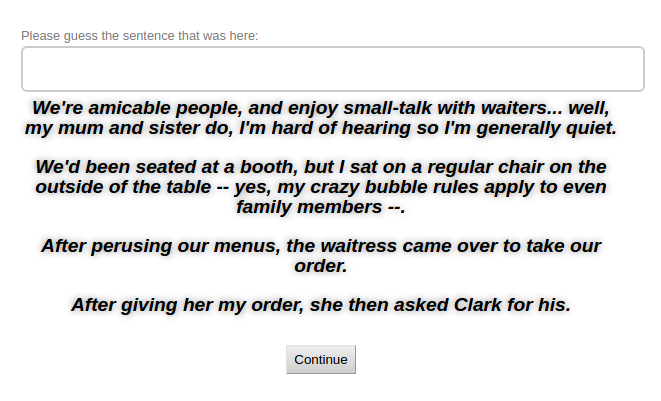
\includegraphics[width=0.35\paperwidth]{images/trial-full-text.png}
  \caption{}
  \label{fig:trial-full-text}
 \end{subfigure}
 \begin{subfigure}{0.4\paperwidth}
  \centering
  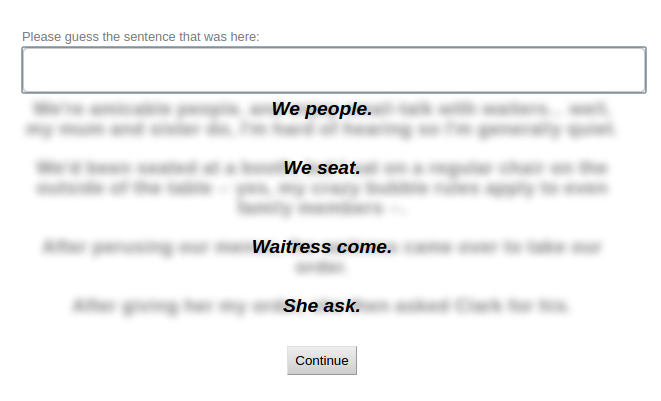
\includegraphics[width=0.35\paperwidth]{images/trial-caveman.png}
  \caption{}
  \label{fig:trial-caveman}
 \end{subfigure}
 \caption{Two example trials, one (a) of the original text condition, the other (b) of the ``caveman'' condition.}
 \label{fig:trial}
\end{figure*}


The models tested by \citeA{rudinger2015learning} had access to only a small amount of linguistic information in the narrative cloze test, since each event was reduced to a single verb and the syntactic role of protagonist.
We wanted to test people's performance on the task under this constraint, but we also wanted to test them on more complex versions of the task, since other more complex models can be tested on narrative cloze tasks with more linguistic information.

We therefore manipulated the original text in three different ways.
In one condition, we gave people the full text of every sentence that contained a mention of the protagonist, which is much more information than the coreference chain models had access to in their version of the narrative cloze task. In a second condition, somewhat resembling the structure of the narrative cloze task used by \citeA{pichotta2014statistical}, we provided people with a ``caveman-speak'' version of the sentence that contained the lemmatized (or participle-form in the case of passive sentences) main verb and a few of its principle arguments: the head of any subject or object noun phrases and the preposition and head noun of any prepositional phrase. For example, the sentence ``Just to spite him, we remained at our table for nearly 3 hours.'' was reduced to ``We remain at table for hours.'' in this condition.
In a third condition, we provided only the main verb and its subject.

\subsection{Procedure}

The format of the task was similar across conditions. We blurred the original text behind each sentence and provided the text for participants on top of this, dependent on condition (Figure \ref{fig:trial}). Above the text box in small letters, we reminded participants to provide a full sentence that they think might have been at that position in the text. In earlier pilots we found that participants sometimes misunderstood the task and gave phrases or fragments instead of sentences. We therefore confirmed that each sentence could be parsed by the CoreNLP tools \cite{corenlp} by running a webserver and parsing participants' responses in real time before accepting each of their responses and allowing them to continue to the next question.

\subsection{Analyses}

\subsubsection{Response processing}

We extracted main verbs from the responses using CoreNLP, and used NLTK's interface to WordNet \cite{bird2009natural, miller1998wordnet} to find all synonyms of that word in all of its synsets. If any verbs or synonym that participants mentioned was the same as the original verb, we recorded that participant's response on that cloze task as correct.
We call this matching method ``automatic matching''.
As this resulted in very low scores, we also manually determined a single word ``gloss'' of each response using the experimenter's subjective judgement. These glosses were chosen generously such that for any set of responses with similar meanings, they were labeled with the same gloss. We consider this a reasonable upper bound on how well participants might be doing on this task.
We call this matching method ``manual matching''.
Given these two metrics for successfully matching the original event, we measured overal performance as the average success for participants across tasks.

\subsubsection{Agreement Metric}

Regardless of whether people are able to recover the actual underlying text, we were also interested in how consistent people's responses might be in tasks like this.

To do this we need to a quantity to represent ``agreement''. We calculated an empirical entropy of the sample distribution of human responses
%(we use a naive entropy, with $P(response) \approx \hat{P}(response) := \frac{N_{response}}{N_{total}}$)
for each cloze task. We first find a gloss for each response, which we determine by finding the root verb and then choosing the name corresponding to that verb's first WordNet synset's.
Given these responses, we cacluate the spread by use a boostrap correction to a naive estimate of entropy \cite{dedeo2013bootstrap}, which is less biased than a naive estimate alone (in which $P(response) \approx \hat{P}(response) := \frac{N_{response}}{N_{total}}$).
However, since different conditions had different total numbers of participants, this quantity alone would be a poor representation of the spread of responses. For example, if 2 participants gave a total of 2 unique responses our sample distribution of responses would have the same calculated entropy as if 5 of 10 participants gave one response and the other 5 gave another. Intuitively, the latter represents clearer agreement among participants than the former, and so we divide this empirial entropy by its maximum possible value for that set of participants. Our measure of agreement is the additive inverse of this scaled entropy, namely:

$$\mbox{agreement} := - \frac{\hat{H}(R)}{\log(N)}$$

where $N$ is the number of participants for that task and $\hat{H}(R)$ represents the entropy estimate across responses for the task. This metric is not defined if N=1, and so we exclude the task and linguistic condition combinations in the pilot for which we collected only 1 participant's response.

The agreement metric tracks humans' intuition rather than the original text, and in this respect it is similar to the metric used by \citeA{pichotta2016learning} for evaluating their model's performance, since they also elicited people's judgements about held-out events. But rather than ask participants to generate narrative cloze answers, they asked participants to judge the {\em model's} top-ranking answers, and so they did not get as much information about what human performance might look like on this task.
%They showed that their LSTM's candidate responses received an average rating of 3.67 on a 0 to 5 rating scale.

\subsubsection{Single-entity Event Chain Model Comparison}

We compare the human data to the single-entity event chain model of \citeA{chambers2008unsupervised}. In this model, the authors select corefference chains of events using Stanford CoreNLP's dependency parser \cite{corenlp,depparse}. They construct a coocurrance matrix between all pairs of events, where an event is a tuple of a main verbe and the role of the coreferenced entity (e.g. subject, direct object, object of prepositional phrase). Events are said to coocur if they are in the same coreference chain, that is if their main verbs have a correferring entity shared across the arguments of those roles. Once the coocurrance matrix is constructed, core script-like knowledge can be characterized by clusters of events. These models approach the narrative cloze task by chosing an event by maximizing the average pointwise mutual information between the target event and all of the context events provided in the narrative cloze task, with some discounting to penalize low occuring words. For the sake of evalution of this inference, the authors looked only at verbs.
% find narrative relations between events (evaluate with narrative cloze task)
% each protagonist offers a different perspective on the narrative chain
% find a partial ordering (evaluate with order coherence metric)
% prune and cluster event chains
% Script representation:
% A narrative chain is a collection of events with a common protagonist. From each document, the entity involved in the most events was selected as the protagonist. Events are pairs of verbs and the semantic role of the protagonist for that verb. Chains of events are learned when the same entity is repeated across multiple verbs. Pairwise relations between events are learned based on how often two events share an argument.
% For example, for the text below:
% McCann threw two interceptions early.
% Toledo pulled McCann aside and told him he’d start.
% McCann quickly completed his first two passes.
% The events where McCann is the protagonist are (threw subject), (pulled object), (told object), (start subject), (completed subject). The more these verbs share the role of the protagonist (i.e. the protagonist of a given document is both the object of pulled and the object of told), the better a script is that contains (pulled object) and (told object), and so the more likely it is that the model will fill in (told object) in a cloze task where the model sees (pulled object). The model ends up learning clusters of events that tend to co-occur. The order of these events is inferred based on syntactic features like tense and uses Timebank for supervised data. (This is based on work in Chambers et al., 2007). The scripts we end up with are directed graphs where nodes are events involving a protagonist and edges are "before" relations.

\citeA{rudinger2015learning} helpfully provided code for this model that we were able to use with only slight modification.
We run the model with the maximum likelihood parameters from \citeA{rudinger2015script}'s experiments.
While this is not the most recent or successful model of its kind, it performed well among the models tested by \citeA{rudinger2015script} and provides an interesting comparison to the human performance.

The model produces ranked lists of candidate events, and various metrics have been adopted for assessing performance.
% could throw some citations in here
One common metric is recall of the actual event within the top N candidates (different papers use different thresholds). Another metric is to determine the model's ranking of the actual event. Because we want to measure against the original text but also against the varied responses that participants gave, we would like a metric of success that considers a set of correct events, rather than a single correct event. We therefore chose, among the set of ``correct'' events, the highest ranking event\footnote{Taking the average of the rankings yielded similar results.} and used its rank to represent the model's performance on that task. For tasks where none of the correct events were recalled, the ranking 100 is used for graphing.

\subsection{Results \& Discussion}

Overall, as \citeA{chambers2008unsupervised} predicted when they introduced this task, people do not perform very well at recovering the original left-out event from an event chain. On average across tasks, people recover the main verb or one of its synonyms 5\% of the time. There is no significant difference between linguistic conditions for this metric (p>0.05). The experimenter's manual judgements showed that people might be able to recover the gist of the original text as much as 8\% of the time. When we use the experimenter's judgement as the metric for success, we actually do find a significant improvement in performance in the condition where the contextual sentences are provided in their original detail (b=0.045, t(2, 126)=3.31, p=0.001). These results are shown in Figure \ref{fig:human-cloze}.

\begin{figure}
 \centering
 \includegraphics[width=0.4\textwidth]{images/human-cloze.png}
 \caption{Human performance on the narrative cloze task is quite poor across trials and across all three linguistic conditions. This is the case even when responses are manually glossed into categories by the experimenter, however with this metric performance is slightly higher when the original text is provided.}
 \label{fig:human-cloze}
\end{figure}

When we measured agreement between participants rather than success at recovering the actual event, the advantage from linguistic detail is no longer apparent (p>0.05 with both automatic and manual tagging). However, participants agreed with one another according to this metric slightly more often than they recovered the original text (8\% with automatic tagging, 11\% with manual tagging). These results are shown in Figure \ref{fig:human-model-comparison}.

% [1] "with  manual  tagging, original condition is no better than the other two:"
%     Estimate   Std. Error      t value     Pr(>|t|) 
% -0.002764528  0.017437071 -0.158543140  0.874322197 
% [1] "with  manual  tagging, average agreement: 0.11"
% [1] "degrees of freedom: 3,109"
% [1] "with  automatic  tagging, original condition is no better than the other two:"
%    Estimate  Std. Error     t value    Pr(>|t|) 
% -0.01041793  0.01382334 -0.75364777  0.45268564 
% [1] "with  automatic  tagging, average agreement: 0.079"
% [1] "degrees of freedom: 3,109"

% From these findings, it seems likely that improvement at the narrative cloze task would not translate to human-like performance and even a model with human-level commonsense would likely do poorly at the narrative cloze task.
These findings suggest that success at narrative cloze tasks does not easily translate to having human-like commonsense knowledge.

\begin{figure}
 \centering
 \includegraphics[width=0.4\textwidth]{images/human-agreement.png}
 \caption{Human agreement on the narrative cloze task is quite low across trials and across all three linguistic conditions. This is the case even when responses are manually glossed into categories by the experimenter.}
 \label{fig:human-agreement}
\end{figure}

We also compared \citeA{chambers2008unsupervised}'s model's minimum rank applied to a ``correct'' response (either a synonym of the actual underlying response or a synonym of a response participants gave) to human agreement and found no significant correlation (p>0.05). That is, the model is not clearly improving in how much it tracks the original text or human intuition as humans become more consistent with one another in their responses.

One potential issue with comparing the min rank metric for model performance to human agreement is that when there are more words to compare to, the minimum rank is likely to be lower. When human responses are used as a source of correct words to compare to, the correlation between human agreement and model min rank variables might be underestimated, since lower agreement might implies more unique words. However, this is not a concern when the source of comparison is the original response or when model ranking is compared to human performance as opposed to agreement, which yield similar results.

% [1] "human agreement is not correlated with model responses"
% 
% 	Pearson's product-moment correlation
% 
% data:  min.rank and human.agreement
% t = 0.10034, df = 66, p-value = 0.9204
% alternative hypothesis: true correlation is not equal to 0
% 95 percent confidence interval:
%  -0.2267430  0.2500386
% sample estimates:
%        cor 
% 0.01234972 
% 
% 
% 	Pearson's product-moment correlation
% 
% data:  min.rank and human.agreement
% t = 0.076462, df = 25, p-value = 0.9397
% alternative hypothesis: true correlation is not equal to 0
% 95 percent confidence interval:
%  -0.3668549  0.3930209
% sample estimates:
%       cor 
% 0.0152907 

\begin{figure}
 \centering
 \includegraphics[width=0.4\textwidth]{images/human-model-comparison.png}
 \caption{The model does not appear to increase in its ability to recover at least one synonym of the humans' responses as agreement between participants increases. Tasks where no human responses were recalled by the model are given the placeholder ranking 100.}
 \label{fig:human-model-comparison}
\end{figure}

\section{Discussion}

\todo{intoduce discussion}

In response to recent concerns about the effectiveness of narrative cloze tasks for specifically targeting commonsense knowledge, \citeA{mostafazadeh2016corpus} very recently developed a dataset with an alternative evaluation metric, a {\em story} cloze task in which models must determine the conclusion of a crowdsourced 4-sentence story segement, and \citeA{pichotta2016learning} chose to extend their narrative cloze tasks so that the model's inferences were compared to people's inferences about what might have been the held-out event.

\subsection{Future Directions}

The clearest next steps for this project would be to increase the number of participants in order to get a more representative view of people's performance on these tasks.

In addition, there have been many more models used for script induction since \citeA{chambers2008unsupervised}, and it may be that the performance of these more recent models might track the performance or agreement of people in our experiment. There is some work collecting human judgements of model candidates that suggests that some models track human intuition at least to some extent even if they do not perform especially well at recovering the original text \cite{pichotta2016learning}.

While natural language is readily available in vast quantities on the internet, sentences that people freely generate tend to be very complex and can often mention events or ideas outside the story they are telling. These features of natural language make both script induction and narrative cloze tasks difficult. For this reason, there have been efforts to use crowdsourcing to collect corpora of stories that are more focused, shorter, and contain more simple language \cite{li2013story, mostafazadeh2016corpus}. \citeA{li2013story} collected stories focused on particular topics (a trip to a restaurant, a bank robbery, etc.) for which they asked the story writers to use very simple language and then recruited readers to identify and exclude mentions of unrelated events. \citeA{mostafazadeh2016corpus} crowdsourced a slightly different, highly structure corpus of 5-sentence-long stories. These stories span a huge variety of commonsense domains, as story writers were told to write about anything they thought readers would easily understand.

It could be argued that given sufficiently curated corpora, narrative cloze tasks would be easier for humans and their success reflective of their commonsense knowledge. One possible test of this would be to repeat all of our analyses on these more simplified crowdsourced corpora.

\todo{state the intended takeaway}

% \todo{Also, we could use word2vec, glove, or sentence2vec embeddings to check similarity between people's responses, though since manually annotating the responses didn't seem to change the results, that might not be all that worthwhile.}

% \todo{more simulations}

% \section{Acknowledgments}

% j s mcdonnel, cocolab, cohort, allen

\bibliographystyle{apacite}

\setlength{\bibleftmargin}{.125in}
\setlength{\bibindent}{-\bibleftmargin}

\bibliography{fyp}

\subsection{Appendix: Illustrative Simulations}

We performed a few different simulations of the narrative cloze task, assuming a tow ``toy'' domains with "scripts" that we hand wrote. We chose the domains to have repeated and dependent structure. In one domain (Figure \ref{fig:video-game-script}), a character plays a video game until they win or get bored. If they lose any level, they return to the first level, and so many aspects of the story might be repeated many times and some events are more or less probable in different contexts. In another domain (Figure \ref{fig:route-to-school-script}), a character travels from home to school, so their route at any given point depends on their previous decisions, and some parts of routes are more or less unique to different overall paths. The scripts for these domains form generative models of possible event sequences. Example event sequences and corresponding informative stories are shown in Table \ref{tab:sampled-stories}.

\begin{figure}
 \centering
 \begin{subfigure}{0.45\linewidth}
  \centering
  \includegraphics[width=0.8\textwidth]{images/video-game-transitions.png}
  \caption{}
  \label{fig:video-game-script}
 \end{subfigure}
 \begin{subfigure}{0.45\linewidth}
  \centering
  \includegraphics[width=0.9\textwidth]{images/route-to-school-map.png}
  \caption{}
  \label{fig:route-to-school-script}
 \end{subfigure}
 \caption{Two toy domains for our narrative cloze task simulations: (a) A video game where levels get more and more difficult and players must start over at level 1 when they lose. Not depicted is the possibility that a player gets bored, which becomes more and more likely with time. (b) A possible map representing a person's possible routes from home to school. Not depicted is the possibility that they might either walk or bike with equal probability.}
 \label{fig:scripts}
\end{figure}

% \begin{table}[bt]
% \begin{center}
% \scriptsize
% % \tiny
% \begin{tabular}{l l l l}
% \toprule
% & Source & Correct Target & Incorrect Target \\
% \hline
% %% coocurrences
% %% model trained on validation succeeds at this:
%     & Kori liked to dress up for comic conventions.
%     & She was very happy when she \textbf{won first place}.
%     & She decided to go to the ballet. \\
% & She decided to dress up as her favorite character \\
% 1 & for an upcoming one. \\
% & She \textbf{worked very hard} for months on her costume. \\
% & She \textbf{entered} the cosplay \textbf{contest} at the convention  \\
% \hline
% %%% causal relations
% %% model trained on validation succeeds at this:
%     & Janet was attending her last year at a university.
%     & Janet's studying paid off and \textbf{she passed}
%     & Janet \textbf{dropped out} of university. \\
% & She wanted to \textbf{maintain her high GPA.} & the exams swimmingly. \\
% 2 & Janet's professor told her that upcoming exams could \\
% & impact her GPA. \\
% & Janet \textbf{began studying} for an additional two hours \\
% & each day. \\
% % causal relation: working harder causes good grades, not dropping out
% % ...or so they say....
% \hline
% %%% agents' goals
% %% model trained on validation succeeds at this:
%     & Sara really \textbf{wanted a new dress} for prom.
%     & Sara had no skills and the \textbf{dress} was a mess.
%     & Sara successfully made some \textbf{pants}. \\
% 3 & However she could not afford one. \\
% & She decided to make her own. \\
% & She gathered the materials and set to work. \\
% \hline
% %%% causal relations
% %% model trained on validation succeeds at this:
% % 4
% %     & Six year old Joe came home with ripped pants.
% %     & Joe admitted it was all his \textbf{fault}.
% %     & Joe said nothing special happened that day. \\
% % & He also gave his parents a note saying he had \textbf{misbehaved}. \\
% % & Joe's \textbf{father yelled at him}. \\
% % & Joe's mother gave him a hug and \textbf{asked for an explanation}. \\
%     & My niece just got engaged.
%     & My niece was \textbf{very upset} that her fiance
%     & My niece was \textbf{thrilled} that her fiance \\
% & She is Chinese and her fiance is Caucasian. & was sick. & was sick. \\
% 4 & Her parents had them over for a home cooked meal. \\
% & The fiance got nausea from the unfamiliar dishes \\
% & and had to leave. \\
% % \hline
% %     & 
% %     & 
% %     &  \\
% % &  \\
% % &  \\
% % &  \\
% \hline
% \bottomrule
% \end{tabular}
% \end{center}
% \caption{ Example Story Cloze Tasks from Mostafazedeh et al. \shortcite{mostafazadeh2016corpus}. Example 1 depends on coocurrances of the events and features in the story and possible answers. Example 2 involves knowledge of causal relations. Example 3 involves knowledge of goals. Example 4 involves some understanding of social and ethical norms. Example 5 demonstrates a common choice between one ending that would make the whole story overall positive, and one that would not.
% %For all of these examples, the correct answer is correctly classified by our proof-of-concept model.
% }
% \label{tab:sampled-stories}
% \end{table}


We model an informative storyteller and an uninformative storyteller. The uninformative storyteller samples a subset of events to describe uniformly from the event sequence. The informative storyteller is a rational speach act model \cite{} where \todo{the meaning of an event is that it happened but other unmentioned events might have to be inferred.} This storytelling model depends on a literal listener model, which infers other events that might have occurred in between the mentioned events such that the whole event sequence could be generated plausibly from the generative model and all of the events mentioned by the speaker occurred in the relative order that they were mentioned.

We test a model of pragmatic reasoning on whether it can infer \todo{a target left-out event from a story}.

Perhaps unsurprisingly,
a rational model that infers left-out events from a story does worse when the story was generated by an informative storyteller than when the story is just a random subsequence of events (see Figure \ref{fig:cloze-simulation}.
We also show that this model does not have much difficulty inferrin events that {\em weren't mentioned} by an informative storyteller, which is the actual task that people observed that script-like knowledge might explain and which inspired the narrative cloze task.

The two two domains both display the property that events mentioned in informtaive stories are harder to recover than unmentioned events in those stories, or mentioned events in uninformative stories. However, there are differences between domains in the recoverability of events overall. It would be interesting to parametrically manipulate the structure of event sequence generative models and show how narrative cloze performance and recovery of unmentioned events varies with properties of the domain (e.g. complexity of causal and/or correlational relationships, repetitiveness, consistency, etc.). It would also be interesting extend these storytelling models to predict discourse markers like ``and'', ``but'', ``so'' and ``because'', perhaps by embedding counterfactual inferences over possible events that could have been in the story.

\end{document}
